%-----------------------------------------------------------------------------%
\chapter{\babTiga}
%-----------------------------------------------------------------------------%

%-----------------------------------------------------------------------------%
\section{Desain Sistem}
%-----------------------------------------------------------------------------%

Untuk dapat menghasilkan program sesuai tujuan, maka perlu dilakukan desain mengenai sistem secara keseluruhan. Sesuai dengan tujuan dari program yang akan menghubungkan antara Zotonic dan \textit{web services} yang dihasilkan oleh ABS \textit{microservices} maka diperlukan sebuah \textit{script} pada Zotonic untuk menghubungkan keduanya.

\begin{figure}
	\centering
	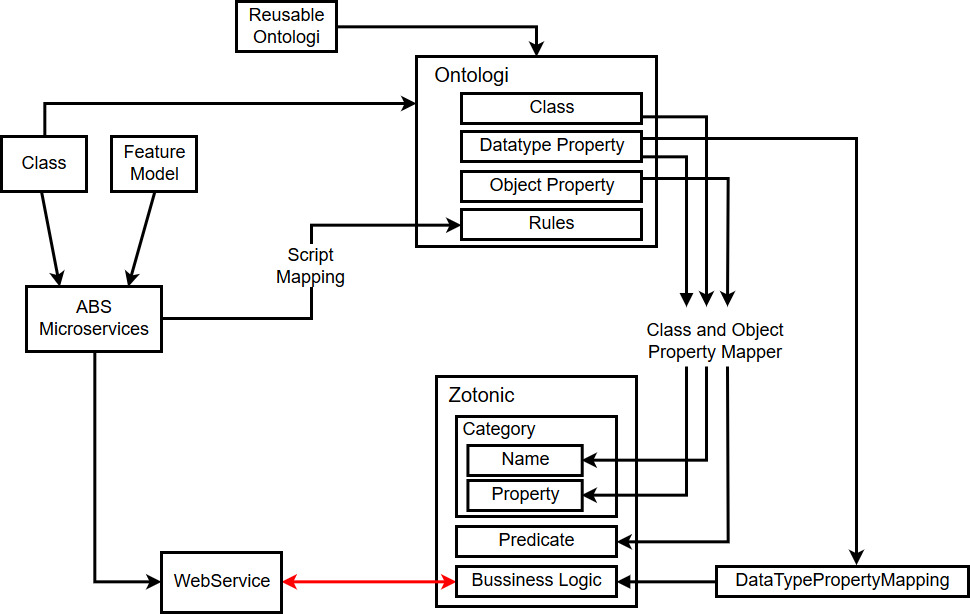
\includegraphics[width=1\textwidth]
		{pics/skripsiRoadmap.jpg}
	\caption{Desain sistem secara keseluruhan}
	\label{fig:skripsiroadmap}
\end{figure}
\vspace{-0.3cm}

Pada \pic~\ref{fig:skripsiroadmap}, terdapat rancangan sistem secara keseluruhan. Pada bagian \textit{Class} dan \textit{Feature Model} untuk menjadi ABS \textit{microservices} telah dilakukan penelitian sehingga penulis tidak perlu melakukan perubahan pada bagian tersebut. Selanjutnya pada bagian ABS \textit{microservices} menjadi \textit{web services} juga telah dilakukan penelitian. Untuk bagian pemetaan dari \textit{Class} menjadi sebuah ontologi dan pemetaan dari ABS \textit{microservices} yang dihasilkan dari \textit{Class} dan \textit{Feature Model} menjadi \textit{Rules} pada ontologi sedang dilakukan penelitian namun hal tersebut tidak menjadi bagian dari penelitian penulis. \\

Untuk bagian pemetaan dari ontologi ke dalam Zotonic telah dilakukan penelitian. Berdasarkan hasil penelitian tersebut, \textit{Class} pada ontologi akan dipetakan menjadi nama dari \textit{Category} pada Zotonic menggunakan \textit{script} classAndObjectPropertyMapper.sh. \textit{Datatype Property} pada ontologi akan dipetakan menjadi \textit{property} dari \textit{Category} yang didapatkan dari \textit{class} pada ontologi menggunakan \textit{script} classAndObjectPropertyMapper.sh. \textit{Object Property} pada ontologi akan dipetakan menjadi \textit{Predicate} pada Zotonic menggunakan \textit{script} classAndObjectPropertyMapper.sh. Selain dipetakan menjadi \textit{property} dari \textit{Category} pada Zotonic, \textit{Datatype Property} juga digunakan untuk proses pembuatan \textit{bussiness logic} pada Zotonic namun fungsi dari \textit{bussiness logic} tersebut masih dibuat secara manual langsung pada kode program.

%-----------------------------------------------------------------------------%
\section{Desain \f{Bussiness Logic}}
%-----------------------------------------------------------------------------%
Beberapa perintah yang dapat digunakan untuk mengubah tampilan adalah: 
\begin{itemize}
	\item \bslash f \\
		Merupakan alias untuk perintah \bslash textit, contoh 
		\f{contoh hasil tulisan}.
	\item \bslash bi \\
		\bi{Contoh hasil tulisan}.
	\item \bslash bo \\
		\bo{Contoh hasil tulisan}.
	\item \bslash code \\ 
		\code{Contoh hasil tulisan}.
\end{itemize}

%-----------------------------------------------------------------------------%
\section{Desain \f{Rules}}
%-----------------------------------------------------------------------------%
Beberapa perintah yang dapat digunakan untuk mengubah tampilan adalah: 
\begin{itemize}
	\item \bslash f \\
		Merupakan alias untuk perintah \bslash textit, contoh 
		\f{contoh hasil tulisan}.
	\item \bslash bi \\
		\bi{Contoh hasil tulisan}.
	\item \bslash bo \\
		\bo{Contoh hasil tulisan}.
	\item \bslash code \\ 
		\code{Contoh hasil tulisan}.
\end{itemize}
